\chead{CHAPITRE 6 . SPRINT 4:Gestion des Projets et Équipes}
 
\chapter{Sprint 4: Gestion des Projets et Équipes}
\renewcommand{\mtctitle}{Sommaire}
\minitoc
\newpage
\section*{Introduction}
\addcontentsline{toc}{section}{\protect\numberline{}Introduction}%
Ce chapitre explore les étapes de la Sprint Gestion des Projets et Équipes, avec un accent particulier sur la structuration des projets, la gestion des équipes et des tâches. Nous débuterons par un aperçu du backlog, avant de détailler la conception, la mise en œuvre et d’illustrer le travail effectué à l’aide de captures d’écran.
\section{Objectifs du Sprint}
L’objectif de cette sprint est de permettre au manager de structurer les projets, gérer les équipes, attribuer des tâches, évaluer les performances, et administrer les fichiers liés aux projets.



\section{Spécification des besoins}
\par Dans cette section, nous allons débuter par présenter le diagramme de cas d’utilisation de la sprint, suivi de l’exposition du backlog associé.
\subsection{Diagramme cas d’utilisation du Sprint 4}

 \begin{figure}[H]
    \centering
    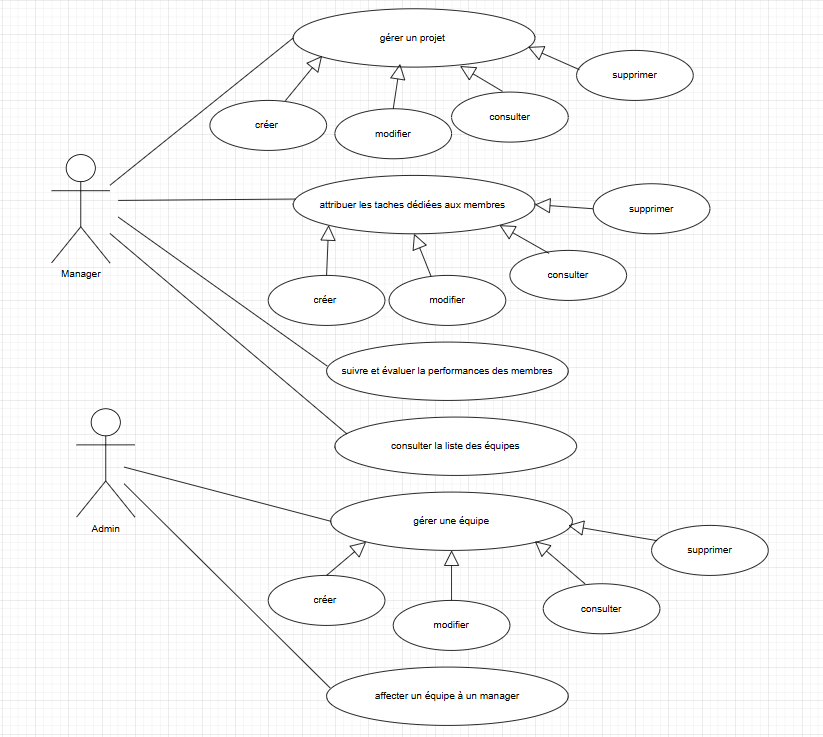
\includegraphics[width=15cm, height=12cm]{Figures/use case 4.png}
    \caption{Diagramme de cas d’utilisation du sprint 4}
    \label{fig:Diagramme de cas d’utilisation du sprint 0}
\end{figure}

\subsection{ Sprint Backlog du sprint 4}
Le tableau ci-dessous présente le sprint backlog établi pour le quatrième sprint. Il récapitule les différentes user stories sélectionnées, accompagnées de leurs identifiants uniques, ainsi que les tâches techniques à réaliser pour chacune. Ce tableau permet d’avoir une vision claire et structurée du travail prévu, en facilitant la planification, la répartition des responsabilités et le suivi de l’avancement tout au long du sprint.
\textbf{\begin{table}[H]
\caption{Backlog du sprint 4}
\centering
\begin{tabular}{|p{1cm}|p{8cm}|p{8cm}|}
\hline
\textbf{ID} & \textbf{User Story} & \textbf{Tâches techniques} \\
\hline
US-17 & En tant que manager, je veux créer, modifier, supprimer des projets afin de structurer mon équipe. 
& 
\begin{itemize}[leftmargin=*]
  \item Concevoir le modèle de données pour les projets.
  \item Créer des interfaces de gestion CRUD.
  \item Implémenter la logique de gestion des projets.
\end{itemize} \\
\hline
US-18 & En tant qu’administrateur, je veux créer, modifier, supprimer une équipe. 
& 
\begin{itemize}[leftmargin=*]
  \item Définir le modèle "Équipe".
  \item Créer les interfaces de gestion.
  \item Gérer les interactions avec la base de données.
\end{itemize} \\
\hline
US-19 & En tant qu’administrateur, je veux affecter une équipe à un manager. 
& 
\begin{itemize}[leftmargin=*]
  \item Ajouter une relation entre équipe et manager.
  \item Enregistrer l'affectation dans la base.
\end{itemize} \\
\hline
US-20 & En tant que manager, je peux consulter les équipes affectées par l’administrateur. 
& 
\begin{itemize}[leftmargin=*]
  \item Développer une interface de visualisation des équipes.
  \item Mettre en place une requête filtrée par manager.
  \item Afficher les données de manière claire.
\end{itemize} \\
\hline
US-21 & En tant que manager, je veux attribuer des tâches aux membres de mon équipe. 
& 
\begin{itemize}[leftmargin=*]
  \item Créer un formulaire d'attribution de tâche.
  \item Lier une tâche à un membre de l’équipe.
  \item Enregistrer l'information dans la base.
\end{itemize} \\
\hline
US-22 & En tant que manager, je veux évaluer la progression des tâches réalisées par les membres de mon équipe. 
& 
\begin{itemize}[leftmargin=*]
  \item Ajouter un champ "état/avancement" dans le modèle tâche.
  \item Créer un tableau de suivi des tâches par membre.
  \item Générer un affichage visuel (ex. barre de progression).
\end{itemize} \\
\hline
\end{tabular}
\label{tab:sprint4_backlog}
\end{table}
}





\section{Analyse des besoins}
Avant de modéliser les fonctionnalités du système, il est essentiel de comprendre les besoins fonctionnels exprimés à travers les différents cas d’usage. La section suivante propose une description textuelle de ces cas d’utilisation, permettant de mieux cerner les interactions entre les utilisateurs et le système, et de poser les bases d’une modélisation cohérente.
    
\subsection{Description textuelle de cas d'utilisation}
   
     \item \textbf{Cas d'utilisation "Gérer un projet": } La table 6.2 ci-dessous présente la description textuelle du cas d'utilisation « Gérer un projet ».

 \begin{table}[H]
 \caption{ Description textuelle du cas d’utilisation "Gérer un projet"}
    \centering
    \begin{tabular}{|c|p{12cm}|}
    \hline
    \textbf{Titre} & Gérer un projet \\
    \hline
    \textbf{Objectif} & Permettre au manager de créer, modifier, supprimer et consulter des projets pour structurer son équipe. \\
    \hline
    \textbf{Acteur}& Manager\\
    \hline
    \textbf{Pré-condition} &Le manager doit être authentifié et avoir les droits d’accès nécessaires.
    \\
    \hline
    \textbf{Post-condition} &Les modifications ou suppressions des projets sont enregistrées dans le système.\\
    \hline
    \textbf{Scénario nominal} & 1. Le manager accède à l’interface de gestion des projets.\newline
    2. Il sélectionne une action (créer, modifier, supprimer).\newline
    3. Il entre ou modifie les détails du projet (nom, description).\newline
    4. Le système valide et enregistre les changements.
    \\
    \hline
    \end{tabular}
    \label{tab:user_stories}
\end{table}

      \item \textbf{Cas d'utilisation "Gérer une équipe": } La table 6.3 ci-dessous présente la description textuelle du cas d'utilisation « Gérer une équipe ».
 \begin{table}[H]
  \caption{ Description textuelle du cas d’utilisation "tableau de bord"}
    \centering
    \begin{tabular}{|c|p{12cm}|}
    \hline
    \textbf{Titre} & Gérer une équipe \\
    \hline
    \textbf{Objectif} & Permettre au manager de créer, modifier, supprimer et consulter des équipes. \\
    \hline
    \textbf{Acteur}& Admin\\
    \hline
    \textbf{Pré-condition} & L'admin doit être authentifié.
    \\
    \hline
    \textbf{Post-condition} & Les modifications ou suppressions des équipes sont enregistrées dans le système.\\
    \hline
    \textbf{Scénario nominal} & 1. L'admin accède à la gestion des équipes. \newline
    2. Il choisit une action (créer, modifier, supprimer).\newline
    3. Il entre les détails (nom de l’équipe, membres, ect.).
    \newline
    4.Le système enregistre les données.\\
    \hline
    \end{tabular}
    \label{tab:user_stories}
\end{table}

      \item \textbf{Cas d'utilisation "Attribuer les tâches aux membres": } La table 6.4 ci-dessous présente la description textuelle du cas d'utilisation « Attribuer les tâches aux membres ».
 \begin{table}[H]
 \caption{ Description textuelle du cas d’utilisation "Attribuer les tâches aux membres"}
    \centering
    \begin{tabular}{|c|p{12cm}|}
    \hline
    \textbf{Titre} & Attribuer les tâches aux membres \\
    \hline
    \textbf{Objectif} & Permettre au manager d’assigner des tâches spécifiques aux membres de son équipe. \\
    \hline
    \textbf{Acteur}& Manager\\
    \hline
    \textbf{Pré-condition} & Une équipe et des tâches doivent exister dans le système.
    \\
    \hline
    \textbf{Post-condition} & Les tâches sont attribuées et visibles pour les membres concernés.\\
    \hline
    \textbf{Scénario nominal} & 1. Le manager accède à la gestion des tâches. \newline
    2. Il sélectionne une tâche et un membre.\newline
    3. Il confirme l’attribution.\newline
    4. Le système met à jour l’assignation.\\
    \hline
    \end{tabular}
    \label{tab:user_stories}
\end{table}

      \item \textbf{Cas d'utilisation "Suivre et évaluer la performance des membres": } La table 6.5 ci-dessous présente la description textuelle du cas d'utilisation « Suivre et évaluer la performance des membres ».
 \begin{table}[H]
 \caption{ Description textuelle du cas d’utilisation "Suivre et évaluer la performance des membres"}
    \centering
    \begin{tabular}{|c|p{12cm}|}
    \hline
    \textbf{Titre} & Suivre et évaluer la performance des membres\\
    \hline
    \textbf{Objectif} & Permettre au manager de surveiller et évaluer la performance des membres de son équipe.. \\
    \hline
    \textbf{Acteur}& Manager\\
    \hline
    \textbf{Pré-condition} & Les membres doivent avoir des tâches assignées.
    \\
    \hline
    \textbf{Post-condition} & L’évaluation est enregistrée et accessible pour consultation.\\
    \hline
    \textbf{Scénario nominal} & 1. Le manager accède à l’interface de suivi. \newline
    2. Il permet de consulter la liste des tâches.\newline
    3. limite l’évaluation aux observations sur le progrès des tâches\\
    \hline
    \end{tabular}
    \label{tab:user_stories}
\end{table}

     \item \textbf{Cas d'utilisation "Affecter une équipe à un manager": } La table 6.6 ci-dessous présente la description textuelle du cas d'utilisation « Affecter une équipe à un managers ».
 \begin{table}[H]
 \caption{ Description textuelle du cas d’utilisation "Affecter une équipe à un manager"}
    \centering
    \begin{tabular}{|c|p{12cm}|}
    \hline
    \textbf{Titre} & Affecter une équipe à un manager\\
    \hline
    \textbf{Objectif} & Permettre à l’administrateur d’affecter un manager à une équipe lors de sa création. \\
    \hline
    \textbf{Acteur}& Administrateur\\
    \hline
    \textbf{Pré-condition} & L’administrateur doit être authentifié et un manager doit être disponible dans le système.
    \\
    \hline
    \textbf{Post-condition} & L’équipe est créée avec le manager assigné et les informations sont enregistrées.\\
    \hline
    \textbf{Scénario nominal} & 1. L’administrateur accède à l’interface de gestion des équipes. \newline
    2. Il crée une nouvelle équipe en entrant les détails (nom, description).\newline
    3. Il sélectionne un manager à affecter à l’équipe.\newline
    4. Le système enregistre l’équipe avec le manager assigné.\\
    \hline
    \end{tabular}
    \label{tab:user_stories}
\end{table}
 
\section{Conception}
\hspace{0.5cm}\textbf Dans cette section, nous discutons de la conception du quatrième sprint. nous Commençons par le diagramme de classes du sprint. Ensuite, nous examinons la modélisation de quelques diagrammes de séquences .  


\subsection{Diagrammes de séquences}
Dans le cadre de l’analyse dynamique du système, un diagramme de séquence a été réalisé pour chaque fonctionnalité clé développée lors des sprints. Le diagramme ci-dessous illustre spécifiquement le scénario du cas d'utilisation « Gérer une équipe », permettant de visualiser les interactions entre l'administrateur et le système lors de la création d’une nouvelle équipe.

\subsubsection{Diagramme de séquence  au cas d’utilisation «Gérer une équipe»}

Cette figure illustre le déroulement du scénario associé à ce cas d'utilisation.
     \begin{figure}[H]
    \centering
    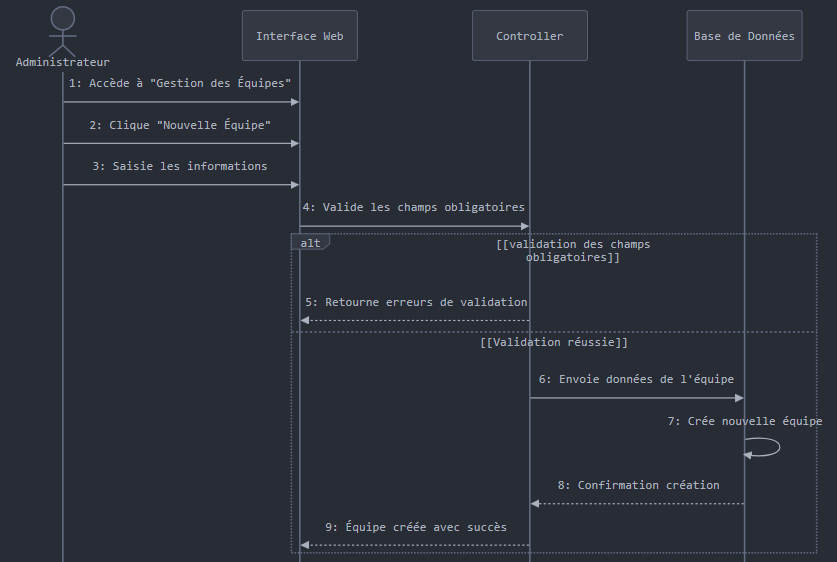
\includegraphics[width=18cm, height=23cm]{Figures/seq4.png}
    \caption{Diagramme de séquence  au scénario « Gérer une équipe »}

\end{figure}

\section{Réalisation: interfaces utilisateur dans HrNova }
CLes interfaces développées dans le cadre de ce sprint permettent aux managers et administrateurs de gérer efficacement les projets, les équipes et les tâches associées. Elles offrent une vue claire sur l’organisation du travail, le suivi des objectifs et la répartition des rôles au sein des équipes.

\vspace{5mm}
\begin{itemize}
     \begin{itemize}
      \item \textbf{Gestion des projets: } Cette interface permet au manager de suivre et gérer les projets. Il peut visualiser la liste des projets, leur statut, leur avancement en pourcentage, ainsi que consulter et modifier les détails de chaque projet, attribuer des équipes et gérer les échéances.
         \begin{figure}[H]
             \centering
             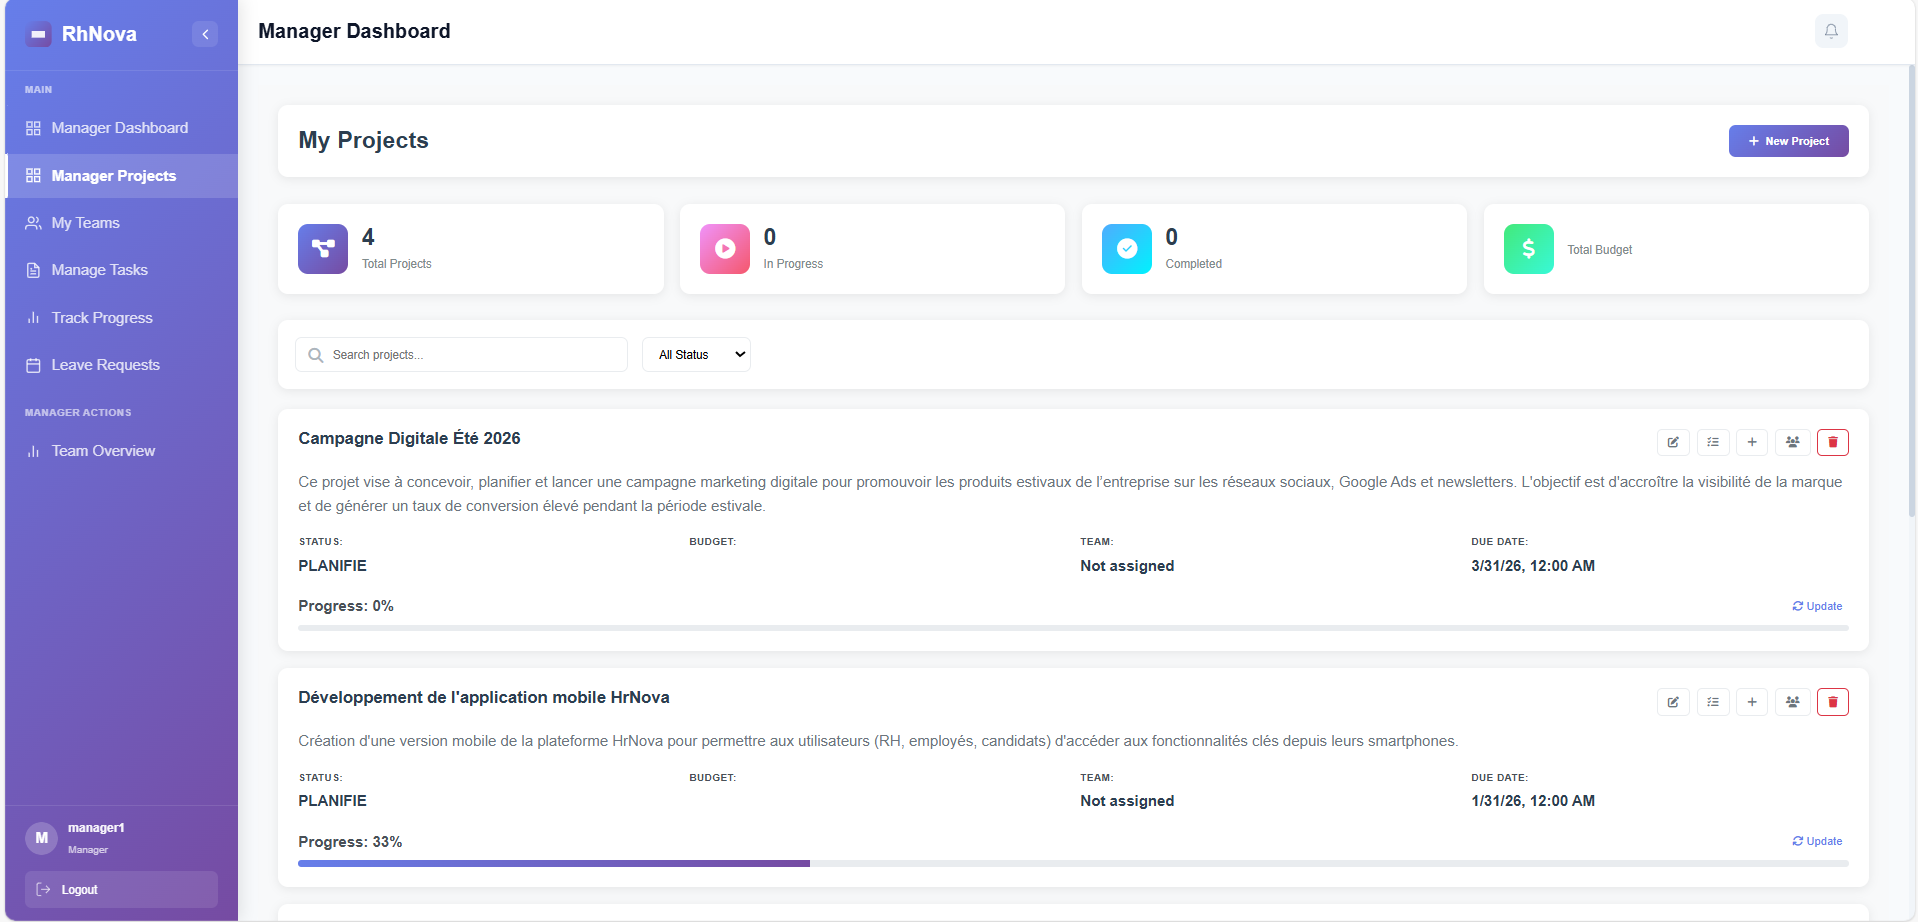
\includegraphics[width=\textwidth]{Figures/managerprojet.png}
             \caption{Page de gestion de projet}
         \end{figure}
     \end{itemize}
\end{itemize}
\begin{itemize}
     \item\textbf{Gestion des tâches : }
Cette interface permet au manager de créer, gérer et suivre les tâches liées aux projets. Il peut définir les priorités, affecter les tâches aux membres de l’équipe, fixer des dates d’échéance, et suivre l’avancement de chaque tâche.
         \begin{figure}[H]
             \centering
             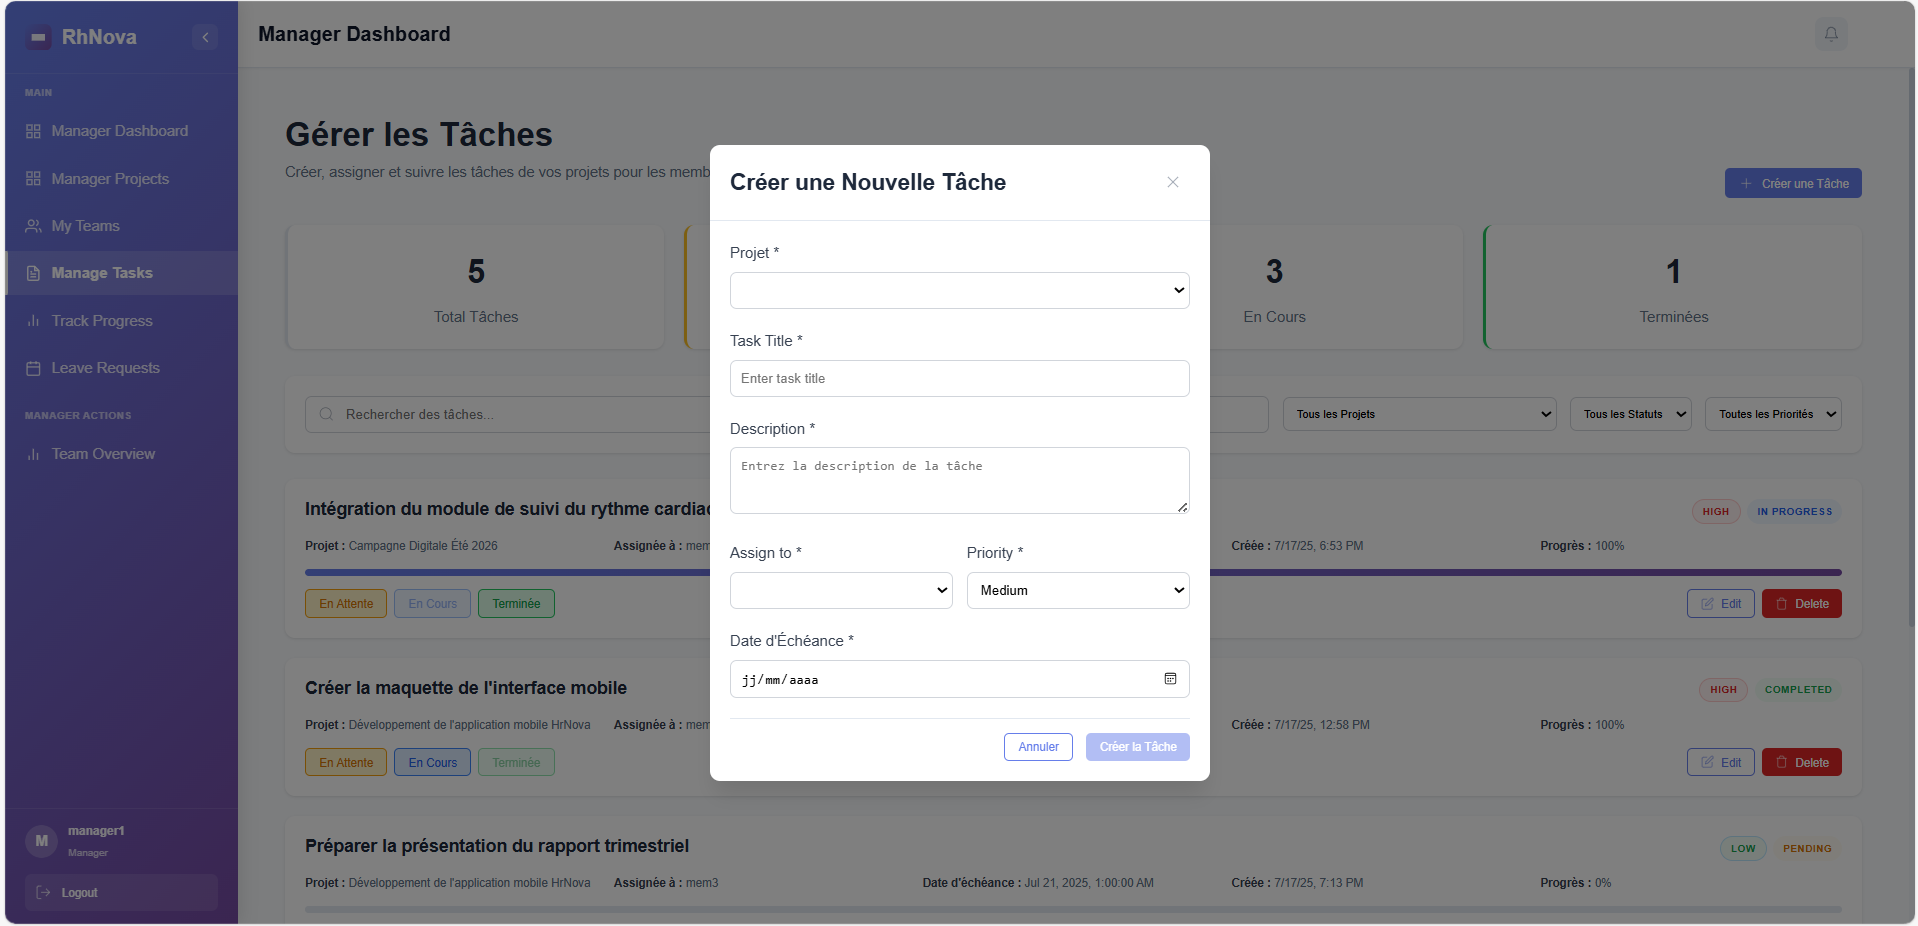
\includegraphics[width=\textwidth]{Figures/managertache.png}
             \caption{Page de gestion des tâches }
         \end{figure}
\end{itemize}  
\begin{itemize}
 \item\textbf{Suivi de la progression : }
Cette interface permet au manager d’évaluer et afin de visualiser l’avancement en direct des tâches assignées aux membres de l’équipe. Elle affiche des indicateurs de performance tels que le nombre de tâches terminées, en cours et en retard, ainsi que le taux de réussite global. Un tableau détaillé liste chaque tâche avec son avancement, sa priorité, son statut, son échéance et le temps passé.
         \begin{figure}[H]
             \centering
             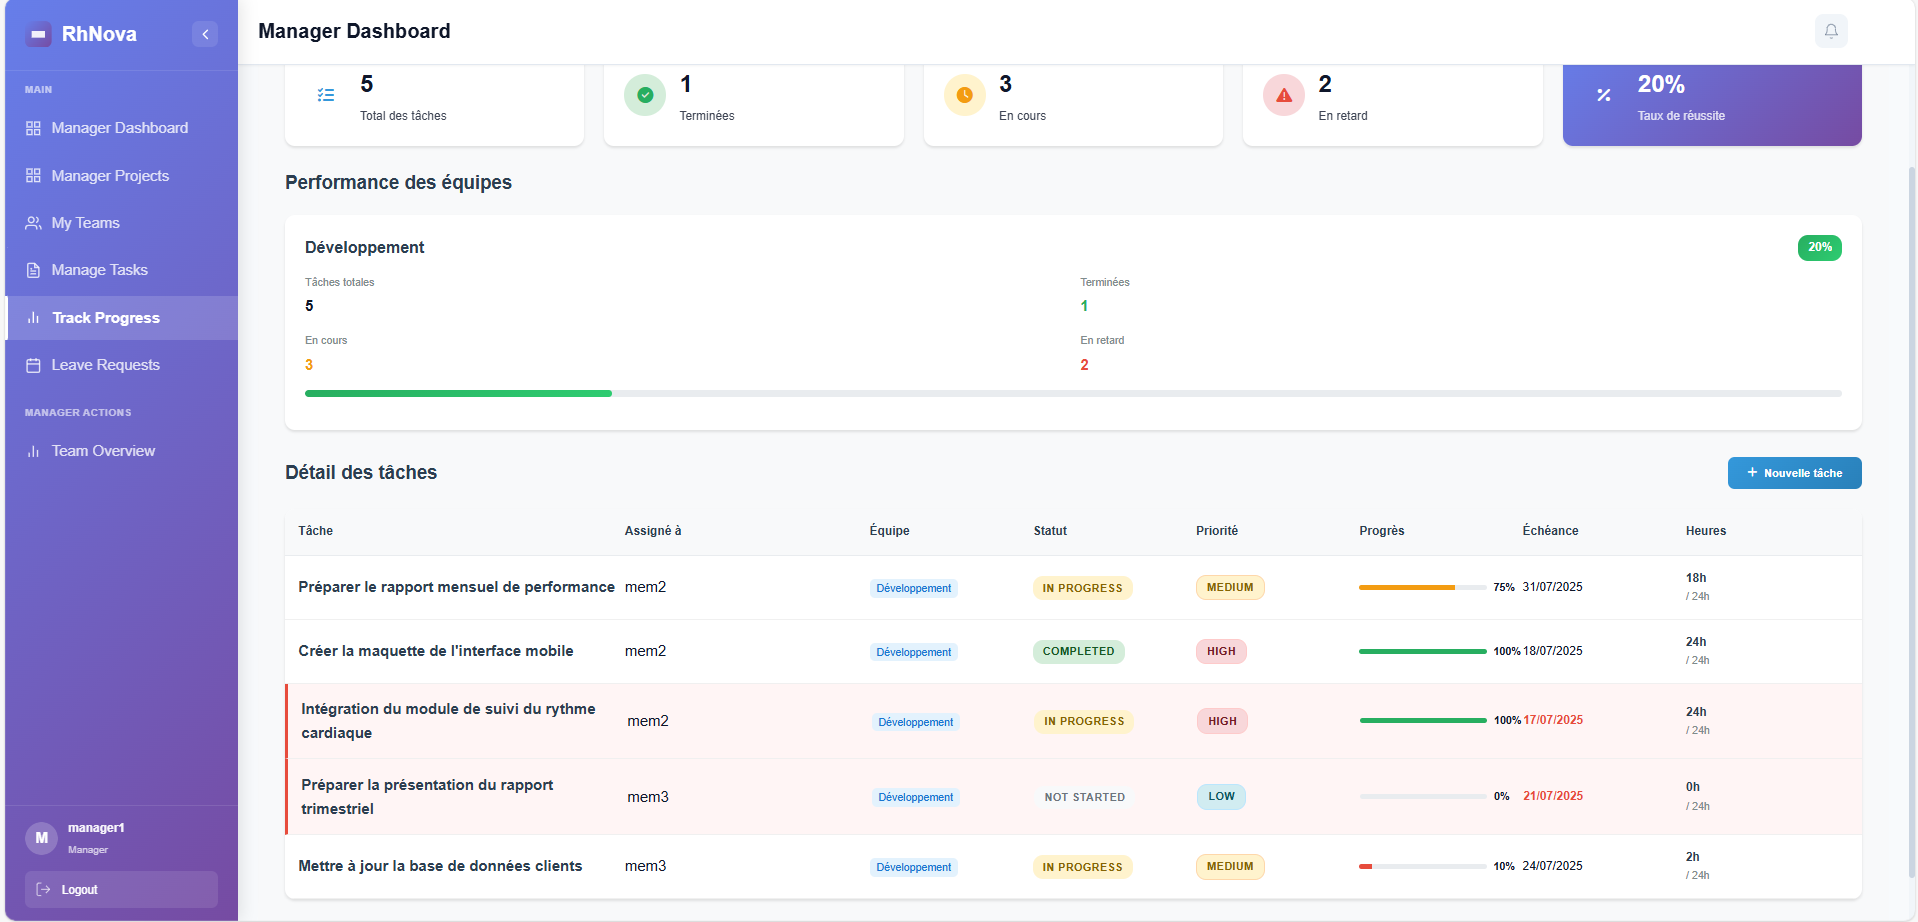
\includegraphics[width=\textwidth]{Figures/managerevalu.png}
             \caption{Page suivi de progression}
         \end{figure}

     \end{itemize}
\begin{itemize}
         \item \textbf{Consultation des équipes : } Cette interface permet au manager de consulter la composition des équipes qui lui ont été attribuées par l’administrateur. 
         \begin{figure}[H]
             \centering
             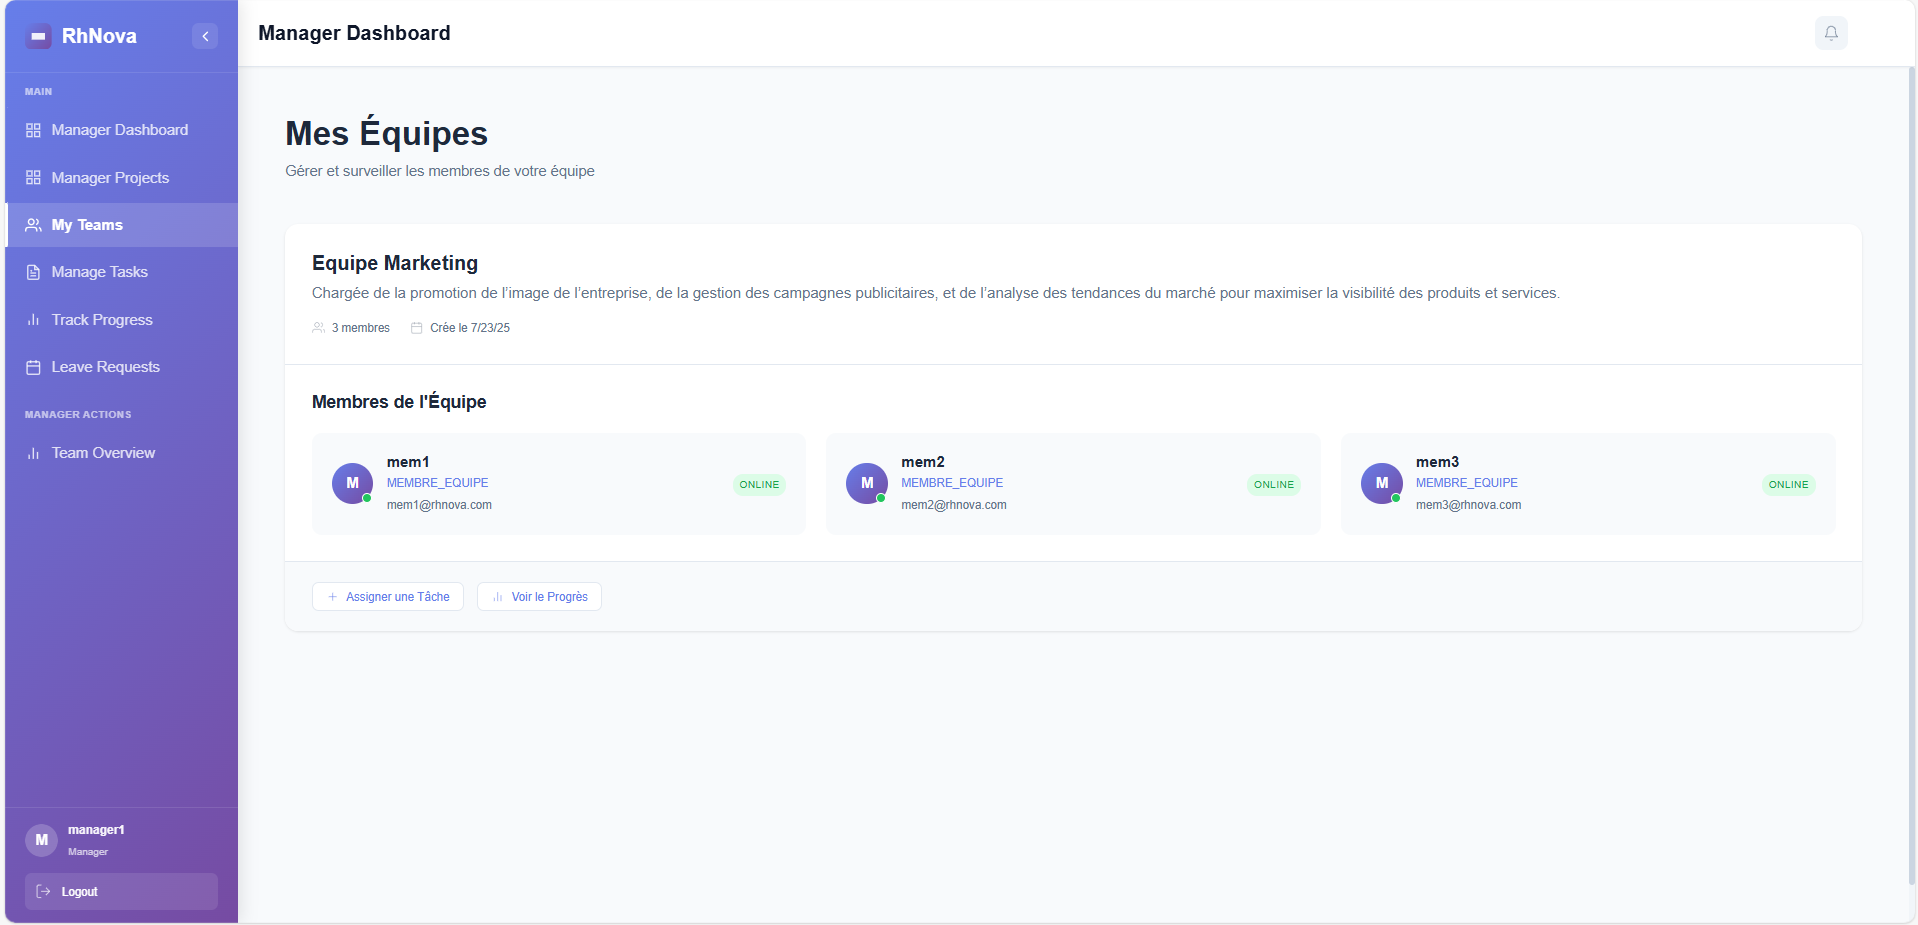
\includegraphics[width=\textwidth]{Figures/managerequipe.png}
             \caption{Page consultation des équipes }
         \end{figure}
     \end{itemize}
\begin{itemize}
         \item \textbf{Gestion des Équipes  : } Cette interface de gestion des équipes est dédiée à l’administrateur. Elle lui permet de créer de nouvelles équipes en renseignant le nom, le manager responsable et une description. 
         \begin{figure}[H]
             \centering
             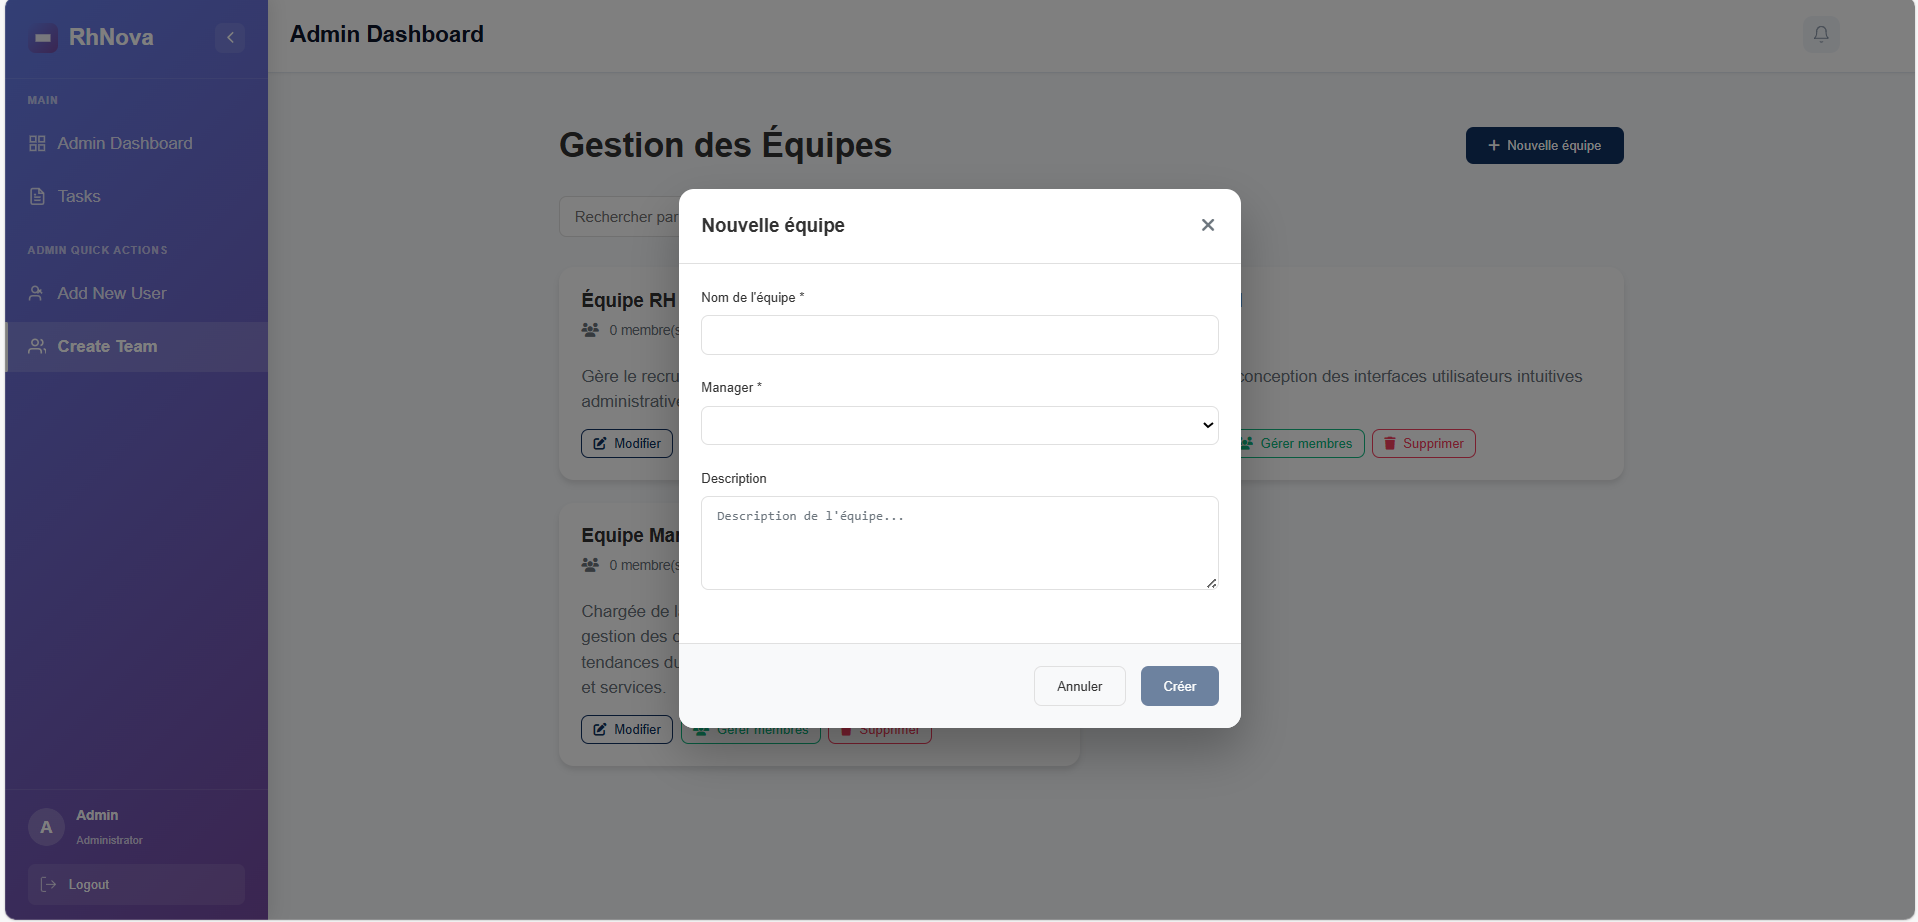
\includegraphics[width=\textwidth]{Figures/admingenerteam.png}
             \caption{Page de gestion des équipes}
         \end{figure}
     \end{itemize}

\section*{Conclusion}
En conclusion, ce chapitre a structuré la Sprint Gestion des Projets & Équipes, en définissant les objectifs et détaillant le backlog, tout en exposant les diagrammes de cas d’utilisation et de classes. Les descriptions textuelles et captures d’écran ont confirmé la mise en œuvre réussie, établissant une base solide pour la gestion des équipes et des projets à venir. Dans le chapitre suivant, nous aborderons les détails du quatrième  sprint " Gestion des Congés et Tâches".
\addcontentsline{toc}{section}{\protect\numberline{}Conclusion}%